\documentclass[fleqn]{beamer}\usepackage[]{graphicx}\usepackage[]{color}
% maxwidth is the original width if it is less than linewidth
% otherwise use linewidth (to make sure the graphics do not exceed the margin)
\makeatletter
\def\maxwidth{ %
  \ifdim\Gin@nat@width>\linewidth
    \linewidth
  \else
    \Gin@nat@width
  \fi
}
\makeatother

\definecolor{fgcolor}{rgb}{0.345, 0.345, 0.345}
\newcommand{\hlnum}[1]{\textcolor[rgb]{0.686,0.059,0.569}{#1}}%
\newcommand{\hlstr}[1]{\textcolor[rgb]{0.192,0.494,0.8}{#1}}%
\newcommand{\hlcom}[1]{\textcolor[rgb]{0.678,0.584,0.686}{\textit{#1}}}%
\newcommand{\hlopt}[1]{\textcolor[rgb]{0,0,0}{#1}}%
\newcommand{\hlstd}[1]{\textcolor[rgb]{0.345,0.345,0.345}{#1}}%
\newcommand{\hlkwa}[1]{\textcolor[rgb]{0.161,0.373,0.58}{\textbf{#1}}}%
\newcommand{\hlkwb}[1]{\textcolor[rgb]{0.69,0.353,0.396}{#1}}%
\newcommand{\hlkwc}[1]{\textcolor[rgb]{0.333,0.667,0.333}{#1}}%
\newcommand{\hlkwd}[1]{\textcolor[rgb]{0.737,0.353,0.396}{\textbf{#1}}}%
\let\hlipl\hlkwb

\usepackage{framed}
\makeatletter
\newenvironment{kframe}{%
 \def\at@end@of@kframe{}%
 \ifinner\ifhmode%
  \def\at@end@of@kframe{\end{minipage}}%
  \begin{minipage}{\columnwidth}%
 \fi\fi%
 \def\FrameCommand##1{\hskip\@totalleftmargin \hskip-\fboxsep
 \colorbox{shadecolor}{##1}\hskip-\fboxsep
     % There is no \\@totalrightmargin, so:
     \hskip-\linewidth \hskip-\@totalleftmargin \hskip\columnwidth}%
 \MakeFramed {\advance\hsize-\width
   \@totalleftmargin\z@ \linewidth\hsize
   \@setminipage}}%
 {\par\unskip\endMakeFramed%
 \at@end@of@kframe}
\makeatother

\definecolor{shadecolor}{rgb}{.97, .97, .97}
\definecolor{messagecolor}{rgb}{0, 0, 0}
\definecolor{warningcolor}{rgb}{1, 0, 1}
\definecolor{errorcolor}{rgb}{1, 0, 0}
\newenvironment{knitrout}{}{} % an empty environment to be redefined in TeX

\usepackage{alltt}

\usefonttheme[onlysmall]{structurebold}
\usepackage[normalem]{ulem} % use normalem to protect \emph
\newcommand\hl{\bgroup\markoverwith
  {\textcolor{yellow}{\rule[-.5ex]{2pt}{2.5ex}}}\ULon}
\usepackage{amsmath,amssymb}
\usepackage{booktabs}
\usepackage{graphicx}
\usepackage{longtable}
\usepackage{lscape}
\usepackage[authoryear]{natbib}
\usepackage{array}
\usepackage{listings}
\usepackage{wasysym}
\usepackage{url}
\usepackage{multirow}
\usepackage{color}
\usepackage{qtree}
\usepackage{inconsolata}
\usepackage{framed}
\definecolor{shadecolor}{rgb}{1,0.8,0.3}
\usepackage[justification=centering]{caption}
\captionsetup{compatibility=false}
\usepackage{subcaption}
\usepackage{xcolor}
\usepackage{hyperref}
\hypersetup{colorlinks=true,linkcolor=blue}
\usepackage[space]{grffile}
\usefonttheme[onlymath]{serif}
\usepackage{sgame}
\usepackage{tikz}
\usetikzlibrary{trees}

\mode<presentation>
\usetheme{boxes}
\usecolortheme{beaver}

\beamertemplatenavigationsymbolsempty
\setbeamertemplate{blocks}[rounded]
\newenvironment<>{block_code}[1]{%
  \setbeamercolor{block title}{fg=white,bg=black}%
  \begin{block}#2{#1}}{\end{block}}

%===================================
% Coloring change
%===================================
\definecolor{darkred}{rgb}{0.8,0,0}
\setbeamercolor{block title}{fg=darkred,bg=structure.fg!20!bg!50!bg}
\setbeamercolor{block body}{use=block title,bg=block title.bg}


\title{Simple Univariate Regression: Part 1}
\everymath{\displaystyle}
\IfFileExists{upquote.sty}{\usepackage{upquote}}{}
\begin{document}
\begin{frame}
\titlepage
\end{frame}






\begin{frame}[c]
  Plan:
  \begin{itemize}
    \item simple univariate regression analysis for the next two weeks
    \item multivariate regression after that
  \end{itemize}
\end{frame}

\begin{frame}[c]
  \frametitle{Population and Sample}
  \begin{block}{Population}
    A set of $ALL$ individuals, items, phenomenon, that you are interested in learning about
  \end{block}
  \begin{block}{Example}
  \begin{itemize}
    \item Suppose you are interested in the impact of eduction on income across the U.S. Then, the population is all the individuals in U.S.
    \item Suppose you are interested in the impact of water pricing on irrigation water demand for farmers in NE. Then, your population is all the farmers in NE.
  \end{itemize}
  \end{block}
  \begin{block}{Important}
    Population differs depending on the scope of your interest
  \end{block}
\end{frame}

\begin{frame}[c]
  \frametitle{Population and Sample}
  \begin{block}{Sample}
    Sample is a subset of population that you observe
  \end{block}
  \begin{block}{Example}
    \begin{itemize}
      \item data on education, income, and many other things for 300 individuals from each State
      \item data on water price, irrigation water use, and many other things for 500 farmers who farm in the Upper Republican Basin (southwest corner of NE)
    \end{itemize}
  \end{block}
  \begin{block}{Question}
    Are the samples representative of the population you are interested in learning about?
  \end{block}
\end{frame}

\begin{frame}[c]
  \frametitle{Econometrics}
  \begin{block}{Econometrics}
    learn about the population using sample
  \end{block}
\end{frame}

% \begin{frame}[c]
%   \frametitle{Econometrics}
%   \begin{block}{The model in the population}
%     The \textcolor{blue}{true} model that governs the data generating process (how the data are generated) in the population
%   \end{block}

% \end{frame}

\begin{frame}[c,fragile]
  \frametitle{Simple linear regression model}
  Consider a phenomenon in the population that is correctly represented by the following model (\textcolor{blue}{This is the model you want to learn about using sample}),
  \begin{block}{A simple model in the population}
  \vspace{-0.6cm}
    \begin{align}
    y=\beta_0+\beta_1 x + u \notag
    \end{align}
  \end{block}
  \begin{itemize}
    \item $y$: to be explained by $x$ (\textcolor{blue}{dependent variable})
    \item $x$: explain $y$ (\textcolor{blue}{independent variable}, \textcolor{blue}{covariate})
    \item $u$: parts of $y$ that cannot be explained by $x$ (\textcolor{blue}{error term})
    \item $\beta_0$ and $\beta_1$: real numbers that gives the model a quantitative meaning (\textcolor{blue}{parameters})
  \end{itemize}
\end{frame}

\begin{frame}[c]
  \frametitle{Simple linear model}
 \begin{block}{A simple model}
  \vspace{-0.6cm}
    \begin{align}
    y=\beta_0+\beta_1 x + u \notag
    \end{align}
  \end{block}
  \begin{block}{What does $\beta_1$ measure?}
  \vspace{-0.6cm}
    \begin{align*}
      \Delta y =\beta_1\Delta x + \Delta u
    \end{align*}
    If you change $x$ by $1$ unit ($\Delta x=1$) while holding $u$ (everything else) constant ($\Delta u=0$),
    \begin{align*}
      \Delta y = \beta_1
    \end{align*}
    That is, $y$ changes by $\beta_1$. We call $\beta_1$ the \textcolor{blue}{ceteris paribus} (with everything else fixed) causal impact of $x$ on $y$.
  \end{block}
\end{frame}



\begin{frame}[c]
  \frametitle{Why do we fish for \textcolor{blue}{ceteris paribus} causal impact?}

  \only<1-1>{\begin{block}{Example: Quality of College}
  You
  \begin{itemize}
    \item have been admitted to University A (better) and B (worse)
    \item are trying to decide which school to attend
    \item are interested in knowing a boost in your future income to make a decision
  \end{itemize}
  \end{block}}

  \only<2-3>{\begin{block}{You have found the following data}
    \begin{center}
    \begin{tabular}{ccc}
           & A & B \\ \hline
    average income         & \multirow{2}{*}{$131$K} & \multirow{2}{*}{$90$K} \\
    after graduation &&\\
    sample size & 500 & 500 \\
    \end{tabular}
    \end{center}
  \end{block}}

  \only<3-4>{\begin{block}{Question}
    Should you assume the difference ($41K$) is the expected boost you would get if you are to attend A instead of B?
  \end{block}}

  \only<4->{\begin{block}{What would you be interested in?}
  Let's say your ability score is $6$ out of $10$ (the higher, the better),
  \only<2->{\begin{align*}
     \;\;\mbox{(1)}\;\; & E[inc|A,ability=9]\\
     & -E[inc|B,ability=6] ?
  \end{align*}}
  \only<3->{\begin{align*}
     \;\;\mbox{(2)}\;\; & E[inc|A,ability=6]\\
     & -E[inc|B,ability=6] ?
  \end{align*}}
  \end{block}}
\end{frame}

\begin{frame}[c]
  \frametitle{Ceteris Paribus Impact of School Quality}
  \begin{block}{Why ceteris paribus impact?}
  \begin{itemize}
    \item you want ability (an unobservable) to stay fixed when you change the quality of school because your innate ability is not going to miraculously increase by simply attending school A
    \item you don't want the impact of school quality to be confounded with something else
  \end{itemize}
  \end{block}
\end{frame}

\begin{frame}[c]
  \frametitle{Why do we want ceteris paribus causal impact?}

\begin{knitrout}
\definecolor{shadecolor}{rgb}{0.969, 0.969, 0.969}\color{fgcolor}

{\centering 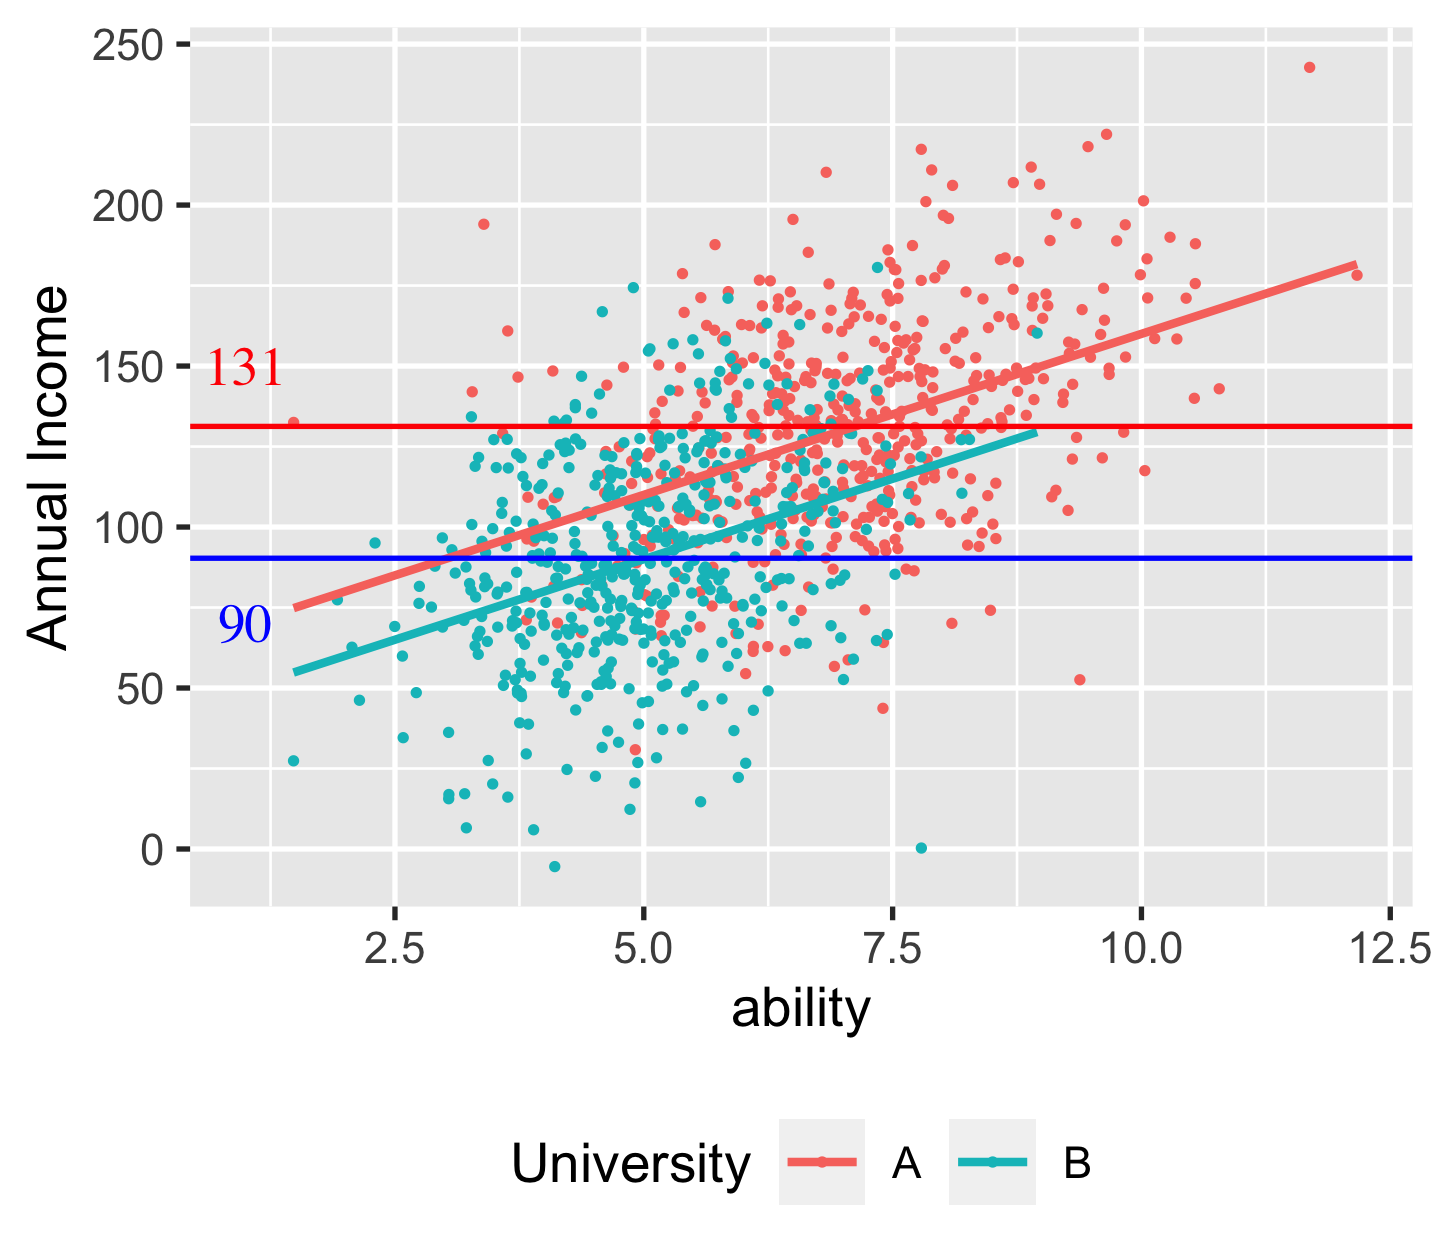
\includegraphics[width=3in,height=3in]{figure/cp-1} 

}



\end{knitrout}

\end{frame}

\begin{frame}[c]
  \frametitle{What does $\beta_0$ measure?}
  \begin{block}{A simple model}
  \vspace{-0.6cm}
    \begin{align}
    y=\beta_0+\beta_1 x + u \notag
    \end{align}
  \end{block}
  \begin{block}{What does $\beta_0$ measure?}
    When $x = 0$ and $u=0$,
    \begin{align*}
    y=\beta_0
    \end{align*}
    So, $\beta_0$ represents the intercept (let's see this graphically).
  \end{block}
\end{frame}

\begin{frame}[c,fragile]
 \frametitle{Graphical representation of the model}

\begin{columns}[onlytextwidth]
  \begin{column}{0.6\textwidth}
\begin{knitrout}
\definecolor{shadecolor}{rgb}{0.969, 0.969, 0.969}\color{fgcolor}

{\centering \includegraphics[width=3in,height=3in]{figure/fig_1-1} 

}



\end{knitrout}
  \end{column}
  \begin{column}{0.4\textwidth}
    \only<2-2>{\begin{description}
        \item [$\beta_0$:] intercept
        \item [$\beta_1$:] coefficient (slope)
    \end{description}}
  \end{column}
​\end{columns}
\end{frame}

\begin{frame}[c]
  \frametitle{Example of a simple linear model}
  \begin{block}{Corn yield and fertilizer}
  \vspace{-0.6cm}
     \begin{align*}
         yield=\beta_0+\beta_1 fertilizer+u \notag
     \end{align*}
   \end{block}
   \begin{block}{Questions}
      \begin{itemize}
        \item what is in the error term?
        \item are you comfortable with this model?
      \end{itemize}
   \end{block}
\end{frame}


\begin{frame}[c]
  \frametitle{Estimating $\beta_1$ using sample}
  \begin{align*}
    yield=\beta_0+\beta_1 fertilizer+u \notag
  \end{align*}

  \begin{itemize}
    \item you do not know $\beta_0$ and $\beta_1$, and would like to estimate them
    \item you observe a series of $\{yield_i,fertilizer_i\}$ combinations ($i=1,\dots,n$)
    \item you would like to estiamte $\beta_1$, the impact of fertilizer on yield, \textbf{ceteris paribus} (with everything else fixed)

  \end{itemize}

\end{frame}

\begin{frame}[c]
  \frametitle{Estimating $\beta_1$ using sample}
  \begin{block}{Question}
    How could we possibly find the \textbf{ceteris paribus} impact of fertilizer on yield when we do not observe whole bunch of other factors (error term)?
  \end{block}
\end{frame}

\begin{frame}[c]
  \frametitle{Crucial conditions to identify the ceteris paribus impact}
  \begin{block}{Before that...}
    You can always assume $E(u)=0$ as long as an intercept is included in the model.
    \begin{align}
        y = & \beta_0 + \beta_1 x + u_1,\;\; \mbox{where}\;\; E(u_1)=\alpha \notag\\
          = & \beta_0 + \alpha + \beta_1 x + u_1 - \alpha\\
          = & \gamma_0 + \beta_1 x + u_2,
    \end{align}
  where, $\gamma_0=\beta_0+\alpha$ and $u_2=u_1-\alpha$. Now, $E[u_2]=0$.
  \end{block}
\end{frame}

\begin{frame}[c]
  \frametitle{Crucial conditions to identify the ceteris paribus impact}
  \begin{block}{Remember}
    You are trying to find the \textbf{ceteris paribus} impact of $x$ (fertilizer) on $y$ (yield), while not observing whole bunch of other factors, $u$
  \end{block}
  It turns out, the following condition between $x$ and $u$ needs to be satisfied,
  \begin{block}{Mean independence (Important)}
  \begin{itemize}
    \item mathematically:
    \begin{align}
      E(u|x)=E(u) \notag
    \end{align}
    \item verbally: the average value of the unobservables is the same at any value of x, and that the common average is equal to the average of $u$ over the entire population
  \end{itemize}
  \end{block}
\end{frame}

\begin{frame}[c]
  \frametitle{Crucial conditions to identify the ceteris paribus impact}
  \begin{block}{Combined with $E(u)=0$}
  \vspace{-0.6cm}
    \begin{align}
      \mbox{mean independence:}\;\; & E(u|x)=E(u) \notag \\
      \Rightarrow  \mbox{\textcolor{blue}{zero conditional mean}:}\;\; & E(u|x)=0 \notag
    \end{align}
  \end{block}
\end{frame}



\begin{frame}[c]
  \frametitle{Correlation and Mean Independence}
  \begin{block}{In practice}
    We use correlation and mean independence interchangeably (though not entirely correct)
  \end{block}
\end{frame}

%--- New Frame ---%

\begin{frame}
  \frametitle{In the context of yield-fertilizer relationship,}
  \begin{align*}
      yield=\beta_0+\beta_1 fertilizer+u \notag
  \end{align*}

  \begin{block}{Questions:}
    (Think about what you would do if you are a famer)
    \begin{itemize}
      \item What's in $u$?
      \item Is it correlated with fertilizer?
    \end{itemize}
  \end{block}
\end{frame}



%--- New Frame ---%

\begin{frame}
  \frametitle{Going back to the college-income example}
  \begin{align*}
    Income = \beta_0+\beta_1 College\;\; A + u
  \end{align*}
  where $College\;\; A$ is 1 if attending college A, 0 if attending college B, and $u$ is the error term that includes ability.
  \begin{block}{Zero conditional mean?}
    \begin{align*}
      E[u(ability)|college A] = 0?
    \end{align*}
  \end{block}
\end{frame}

%--- New Frame ---%

\begin{frame}
  \frametitle{Going back to the college-income example: $E[u|x]\ne 0$}
\begin{knitrout}
\definecolor{shadecolor}{rgb}{0.969, 0.969, 0.969}\color{fgcolor}

{\centering \includegraphics[width=3in,height=3in]{figure/college_income_g-1} 

}



\end{knitrout}
\end{frame}

%--- New Frame ---%

\begin{frame}
  \frametitle{Going back to the college-income example: $E[u|x] = 0$}
\begin{knitrout}
\definecolor{shadecolor}{rgb}{0.969, 0.969, 0.969}\color{fgcolor}

{\centering \includegraphics[width=3in,height=3in]{figure/college_income_g_unbiased-1} 

}



\end{knitrout}
\end{frame}


\end{document}



